\documentclass[11pt,a4paper]{report}
%\usepackage[cm]{fullpage}
\usepackage{enumerate}
\usepackage{graphicx}
\usepackage{fancyhdr}
\usepackage{hyperref}
\usepackage{float,lscape}
\usepackage{longtable}
\usepackage{multirow}
\usepackage{geometry}
 \geometry{
 a4paper,
 total={210mm,297mm},
 left=20mm,
 right=20mm,
 top=20mm,
 bottom=20mm,
 }

\hypersetup{%
	colorlinks=false,% hyperlinks will be black
%	linkbordercolor=red,% hyperlink borders will be red
	pdfborderstyle={/S/U/W 1},% border style will be underline of width 1pt
	linktoc=page% defines which part of an entry in the table of contents is made into a link. Valid values: none,section,page,all
}

\pagestyle{fancy}
\fancyhf{}

\fancyhead[L]{Work Package 1 Application and environment requirements \\ Deliverable D1.1 Natural language requirements}
\fancyfoot[C]{\thepage}
%\rhead{this 
\renewcommand{\headrulewidth}{0.4pt}
\renewcommand{\footrulewidth}{0.4pt}

%\setlength{\textheight}{580pt}

% % % % % % % % % % % % % % % % % % % % % % % % % %
% Aconyms for SyncFree project.
%
% Author: Amadeo Asco
% Last updated: 24 July 2014
% % % % % % % % % % % % % % % % % % % % % % % % % %
% The acronym package helps you manage acronyms and acronym lists in your documents, http://www.mackichan.com/index.html?techtalk/456.htm~mainFrame
% for the glossary to show up in Table of Contents you need to additionally add toc option
\usepackage[toc,nonumberlist]{glossaries}
%\showthe\hsize% interrupts latex and shows value of \hsize
\setlength{\glsdescwidth}{0.82\hsize}%
% to remove extra line between groups
\renewcommand{\glsgroupskip}{}
% To get rid of the full stop after the description in the glossary
\renewcommand{\glspostdescription}{}
\makeglossaries

% Start definitions ---------------------------
% Add all of the definitions for the abbreviations
\newacronym{2i}{2i}{Secondary Indexing}
\newacronym{2pset}{2P-Set}{Two-Phase Set}
\newacronym{acid}{ACID}{Atomicity, Consistency, Isolation, Durability}
\newacronym{b2b}{B2B}{Business to Business}
\newacronym{base}{BASE}{basically available, soft state, eventual consistency}
\newacronym{cci}{CCI}{Causality, Convergence and Intention}
\newacronym{cmrdt}{CmRDT}{Op-based Convergent Replicated Data Type}
\newacronym{cprdt}{CPRDT}{Conflict-free Partially Replicated Data Type}
\newacronym{crdt}{CRDT}{Conflict-free Replicated Data Type}
\newacronym{cqrs}{CQRS}{Command Query Responsibility Segregation}
\newacronym{cvrdt}{CvRDT}{State-based Convergent Replicated Data Type}
\newacronym{dc}{DC}{Data Centre}
\newacronym{ec}{EC}{Eventual Consistency}
\newacronym{ga}{GA}{Genetic Algorithm}
\newacronym{gset}{G-set}{State-based increment-only Counter}
\newacronym{gp}{GP}{General Practitioner}
\newacronym{ha}{HA}{High Availability}
\newacronym{id}{ID}{identifier}
\newacronym{lww}{LWW}{Last-Writer-Wins}
\newacronym{lwwr}{LWW-Register}{Last-Writer-Wins Register}
\newacronym{mdc}{MDC}{Multi Data Centre}
\newacronym{mv}{MV}{Multi-Valued}
\newacronym{mvr}{MV-Register}{Multi-Valued Register}
\newacronym{orset}{OR-set}{Observed-Removed Set}
\newacronym{rdbms}{RDBMS}{Relational Database Management System}
\newacronym{rga}{RGA}{Replicated Growing Array}
\newacronym{rest}{REST}{Representational State Transfer}
\newacronym{rpc}{RPC}{Remote Procedure Call}
\newacronym{cap}{CAP}{Consistency, Availability and Partition tolerance}
\newacronym{sec}{SEC}{Strong Eventual Consistency}
\newacronym{ttl}{TTL}{Time To Live}
\newacronym{uset}{U-Set}{Two-Phase Set with unique elements}
\newacronym{wp1}{WP1}{Work Package 1}
\newacronym{wp2}{WP2}{Work Package 2}
\newacronym{wp3}{WP3}{Work Package 3}
\newacronym{wp4}{WP4}{Work Package 4}
\newacronym{wp5}{WP5}{Work Package 5}
% end abbreviations ---------------------------

%\ifnum\showDefinitions=1
% Add all of the definitions
%\newglossaryentry{bwd}{name={box-and-whisker diagram}, text={box-and-whisker diagram}, first={box-and-whisker diagram},
%    description={\parbox{10.6cm}{\medskip The bottom and top of the box are the 25th and 75th percentile (the lower and upper quartiles, respectively), and the band near the middle of the box is the median, whereas the dot represent the mean. The ends of the whiskers represent the minimum and maximum of all of the data.\medskip}}}
% end definitions -----------------------------
%\fi

\glsdisablehyper

\hypersetup{linktocpage}
% Title
\title{{\Huge SYNCFREE} \\ Work Package 1 Application and environment requirements \\ Deliverable D1.1 Natural language requirements}
%\title{SYNCFREE\\Deliverable D1.1\\Natural Language Requirements}
%\author{Project acronym: SyncFree\\Project Title: Large-scale computation without synchronisation\\Funded by: 7th Research Framework Programme, ICT call 10, grant agreement n°609551\\Issue: 0.1\\Edited by: Tom Benedictus \href{mailto:tob@trifork.com}{tob@trifork.com}}
\author{Project acronym: SyncFree\\Project Title: Large-scale computation without synchronisation \thanks{7th Research Framework Programme, ICT call 10, grant agreement n°609551}\\Issue: 0.1\\Edited by: Tom Benedictus (\href{mailto:tob@trifork.com}{tob@trifork.com})}


\makeglossaries


\begin{document}

\maketitle

\newpage

\tableofcontents{}

\chapter{Introduction}
% \section{Introduction}

Description of the deliverable 1.1 : ``{\em Natural-language
  requirements: Initially, the use cases selected by the project
  partners will be described informally in natural language. Such a
  description consists of an outline of the targeted supporting
  architecture and a list of the informal constraints the system must
  ensure.}''

Six use cases have now been described by the industrial partners in
the SyncFree Project, Table \ref{tb:use_cases}. All use cases are distributed databases having
one or more data centers acting as central authority.
In some use cases, the distributed database also spans mobile devices
being ``sometimes connected'' - both with each other and the central
authority.

The selected use cases are:
\begin{table}[htb] \centering
		\begin{tabular}{| c | l | l | p{8.5cm} |}
			\hline
			Ref. & Application & Provided by & Brief \\ \hline
			1 & Ad Counter & Rovio & Web pages and apps are presenting commercial ads that must be displayed e.g. 100,000 times while not repeated too often on one device.\\ \hline
			2 & Leader Board & Rovio & For each game, records must be available about the leading player. Some players use several devices. \\ \hline
			3 & Wallet & Rovio & Debiting and keeping track of balance is is critical for a stable in-game economy. \\ \hline
			4 & Shared Medical Record & Trifork & Sharing information on a patient's current medication between healthcare professionals and the patient himself. \\ \hline
			5 & \gls{b2b} & Trifork & The ability to present new products, place orders, and keep track of delivery using tablet computers is the basis for this \gls{b2b} application that connects thousands of stores with the manufacturer. \\ \hline
			6 & Festival & Trifork & 10s of thousands of participants in one of the world's largest two week music festivals are concurrently rating their experience and the momentary results are made generally available. \\ \hline
		\end{tabular}
		
		\caption{Use cases.}
		\label{tb:use_cases}
\end{table}
              
The use cases are described following a questionnaire defined
by the project members (See Appendix A).
After presenting the individual use cases we summarize our
observations with conclusion relating this deliverable results to the
other work packages.

\chapter{Use Cases}
\section{Ad Counting}
\subsection{Application description}
Advertising platforms need to accurately record impressions (number of times an ad has been served) and clicks, in order to analyze advertising data. They use distributed counters, which are challenging to implement in a dynamic, fault-prone environment. \gls{crdt} counters are a promising solution; the challenge is to scale to an extreme numbers of users. 
 
Rovio's Ads service keeps track of impressions and clicks for ads per campaign/ad/country. Typically these counts have some upper bound  after which the ad should not be shown anymore. The upper bound may consist of the sum of several counters (e.g show the same ad 50,000 times in the US, 10,000 times in the UK and 100,000 times in total), so it is not really feasible to enforce the upper bound on the data storage layer.

The main use for the tracking data is to control the rate of ads shown to the users. The campaign capacity should be spread evenly over the campaign instead of showing all the impressions during the first hour of the campaign. Therefore, the data must be updated in real time although a good estimate is normally enough.

The Ads service runs on multiple service nodes, which is shown in Figure \ref{fig:add_server}, so in order to avoid write conflicts each of those nodes has its own document for the impression and click counters in Riak. This is already a simplified implementation of the counter \gls{crdt}. The true value of the counter can be obtained by calculating the sum of all counters manually.
\begin{figure}[!h]
	\centering
	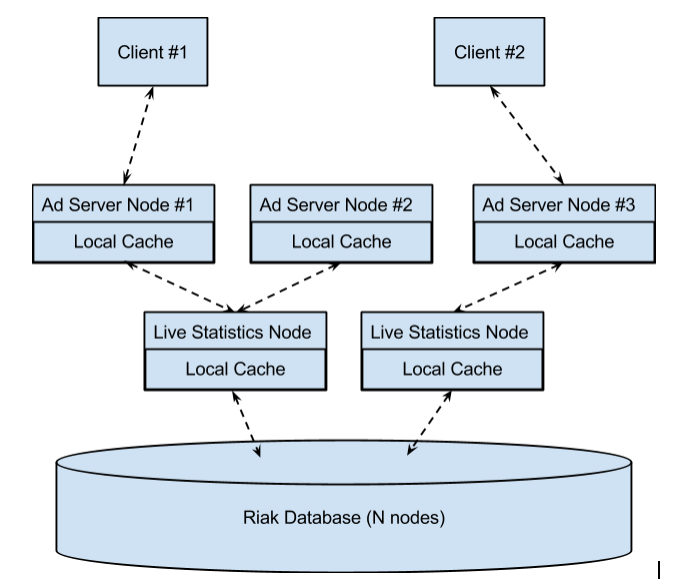
\includegraphics[width=0.7\textwidth]{./img/image1.png}
	
	\caption{Add server.}
	\label{fig:add_server}
\end{figure}

Even if the current solution works, it is neither very elegant nor easy to maintain. The \gls{crdt} counters will provide a more efficient solution for updating the counters. The ad system does not need a strict limit for the counter and we can implement an optimistic solution: if the counter value is less than the limit, show the ad and increase the counter. This may result in showing the ad too many times, but it is ``close enough''. Client applications running on different kind of devices (mobile phones, web browsers etc) connect to the Ads service in order to determine which ads to show to their users. The same ad should not be shown on the same device for more than 3 times a day, so the Ads service keeps track of which device has been shown which ad and when. This data is currently stored in one document that contains information on the ads shown on a device during the last couple of days (basically which ad has been shown and when). It might be possible to utilize \glspl{crdt} in this document, but the current implementation has no major issues, either.

Each server node has its own cache representing the counters. The cache could be dropped theoretically but in practice, it will be needed. The counters get synced between the live statistics nodes via Riak. Each counter will have three replicas on the database meaning the value is formed based on those copies.

The live statistics nodes serve the entire state of all campaigns. They hold a cache for the data and keep it in sync via Riak. There is a local estimation in place between the synchronizations since the data is not synced on every update they get from the ad servers.

The database holds two types of documents:
\begin{itemize}
	\item Live documents for each day that is still missing the verified data from the analytics pipeline. Note that there is one document for each live stats host to avoid conflicts in the database level.
	\item Documents containing the reliable data from the analytics pipeline.
\end{itemize}

There may be a document for the same day in both analytics documents and live documents, Figure \ref{fig:example_temporary sitiation}. This is a temporary situation which gets corrected once the data import process removes the obsolete live document from the database. However, the synchronization process in live stats nodes must be such that it tolerates duplicate documents and ignores the obsolete daily documents.

\begin{figure}[!h]
	\centering
	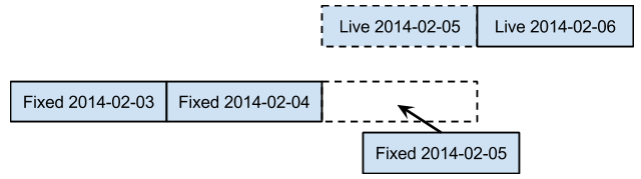
\includegraphics[width=0.7\textwidth]{./img/image2.png}

	\caption{Example of temporary situation.}
	\label{fig:example_temporary sitiation}
\end{figure}

The diagram shows how the document for 2014-02-05 is added to the fixed (data from analytics pipeline) documents and right after that, the live document for 2014-02-05 is removed. There is a small window when both documents exist and the synchronization process must take care of the removal of the duplicates.

\subsection{Conflict situations}
Updating a single counter without any \gls{crdt} solution will not work. Two instances making the update in a sequence of 
\begin{center}
read $\rightarrow$ increase $\rightarrow$ write 
\end{center}

at the same time will cause the updates to overwrite each other or at least make the sibling resolution extremely difficult and unreliable.
For example:
\begin{enumerate}
\item Node A reads value N from the database.
\item Node B reads value N from the database. 
\item Nodes A and B increase the value to $N+n_A$ and $N+n_B$. 
\item Nodes A and B write the values to the database resulting in two siblings. 
\item Node C reads the value from the database $\rightarrow$ two siblings with values $N+n_A$ and $N+n_B$. 
\item Node C is unable to resolve the correct value of the counter with the obtained information $\rightarrow$ data is lost.
\end{enumerate}

Note, this issue has already been solved with the simplified implementation of \gls{crdt} counter.

\subsection{Invariants}
The value of the counter (how many times the ad has been shown) should not exceed the limit. 
The invariant does not need to be strict since the extra times don't really cause any significant harm.

\subsection{Transactions}
N/A

\subsection{Divergence}
\subsubsection{Expected latency}
The latency requirements are not very strict in the ad case. The counters should get converged within some seconds in normal operations to get proper limits in place. However, no real harm is done even if there is a longer split in the cluster.

\subsubsection{Offline mode}
There is no real offline mode but the service nodes must be able to operate even though there is a cluster split in the database layer. For example, if there is no connectivity between two data centers, the service nodes must still be able to operate normally. The counters will be converged as expected when the data centers have the normal connectivity between them.

\subsubsection{Limits to the degree of temporary divergence}
It is ok for us if the counter value is ``wrong'' in two ways:
\begin{itemize}
\item Some updates are missed entirely. This is the worse type of discrepancy since it will mess up the final reporting. If the probabilistic nature of the value is unknown (e.g. varies as a function of the server load), the final values may have an unexpected differences to the correct values.
\item Updates from different nodes are delayed  for a while as the server nodes only sync there counts periodically (every one 1min) but the values are correct eventually. This case is an easier one since the counter is used for checking the limits in real time but the limit does not need to be enforced strictly its ok if we serve slightly more than the limit .
\end{itemize}

\subsubsection{Divergence visibility}
There does not need to be visibility to the divergence in the system. Obviously, there may be a need for identifying if there is a case of a longer cluster split (several hours) but that can be detected from other monitoring utilities.

\subsubsection{Divergence guarantees}
A mechanism for guaranteeing that the data is not more divergent than some specific amount would reduce the issues with showing ads more than needed when there is a cluster split.

\begin{itemize}
\item It would be interesting if the \gls{crdt} system could give an estimate of the number of missing operations on the document. However, the number should not overestimate the real value.
\item The latency of the reads/writes is more important than the correctness of the value in general.
\end{itemize}

\subsection{Partitioning}
Since the impression and click counters are recorded per country, global consistency of the counters across data centers could be lower but a  higher consistency is required in the primary data center for the country the counter belongs to. This would mean that the reports for global campaigns would be consistent with some delay but this shouldn't be a problem.

\subsection{Operational Requirements}
\begin{itemize}
\item The reason for EC: Availability and performance.
\item The application is running on a data center. There is a small possibility of running it on multiple \glspl{dc} later but one \gls{dc} is enough for now.
\item There are three replicas of the data in the database level but the cached values on the server will increase the number of replicas to ``tens''.
\item The data is fully replicated between the cached instances.
\item The number of objects in this use case is currently running in scale of tens of thousands. The count may increase up to hundreds of thousands later.We need 3 counters for each ad in each campaign so the object count will be Number of campaigns * number of ads in the campaign * 3 (each ad has 3 counters associated with it , impressions , clicks and downloads)
\item The object is basically a single counter meaning that the size is in bytes. However, the current structure in the database level is such that there are tons of counters aggregated into a single document.
\item The database is a single big database on the architectural level but it consists of several nodes hosting the different replicas of the data.
\end{itemize}

\subsection{Security Requirements}
\begin{itemize}
\item There is no access control on the lower levels of the system. The end users won't be able to do anything else than increase the number of shown impressions etc. for the specific user.
\item All actions are audited to a flat data storage from which a batch job gathers the data and updates the counter documents accordingly. This process ensures the data integrity on daily level but the process cannot be implemented in real time due to the volumes of data. The batch jobs are run on a nightly basis and they take multiple hours to process and aggregate events for a day.  The process can also be used for rolling back malicious operations in the system if there are any.
\end{itemize}

\subsection{Existing State}
The application is running in production with an implementation that handles the conflict resolution with a custom \gls{crdt} implementation for the counters. Each replica on the application level are written to a separate document and those documents are merged and the aggregated counts are stored in memory the loading phase (when the document is read from the \gls{db} this happens periodically every one min. currently). In practice, it is similar to the counter \gls{crdt} implementation on the \gls{db} layer.

There have been some challenges around how to verify the data integrity if something catastrophic happens (someone deletes a live document etc.). The current implementation handles those issues with a daily-based document structure and a feedback loop from the more reliable analytics data. Analytics events are fired for each ad served and are stored in flat files in s3 . The analytics data contains information about every ad delivery and is the most reliable source of information in the system. This structure will ensure that the documents will be in good shape eventually and the data can be corrected if there is a need to.



\section{Leaderboard}
\subsection{Application description}
Leaderboards are used in games to provide information on who are the best players globally (and often also domestically) and how the current player ranks against other players.
Rovio's Leaderboard service provides different kind of leaderboards for games. The default type of leaderboard is level­-based which means that the high scores are stored by level, so each user has one document per each level passed in a game. Each level score document contains the user's high score, (estimated) rank, matchmaking and percentile indices and some other additional properties the service itself doesn't care about (e.g. stars, lap time etc. depending on the game).
Since the leaderboard should always contain the highest score the user has achieved in a level, custom conflict resolution based on the high score is required. With \glspl{crdt} the conflict resolution could be done so that the maximum or minimum score wins, and the rest of the properties are taken from the update that contained the new score (no conflict resolution required).
The leaderboard service supports the following operations:
\begin{enumerate}
\item Send score (adds or updates the high score of the user)
\item Get ranking (returns the user's ranking in a level)
\item Get matching (returns a list of user IDs whose ranking is close to the requesting user)
\item Get leaderboard (returns the leaderboard for top ranking users, user's friends etc.)
\end{enumerate}

\subsection{Conflict situations}
The same user sending a high score for the same level concurrently is quite unlikely but possible if a level can be passed very quickly or if the same user account is used from two different devices at the same time. In this kind of situation the best score should be persisted so the last write wins resolution (which Riak provides) will not be sufficient.
We have games that can be played offline and they sync their score when they get a connection.In that case the device stores that scores of different levels locally when offline and then update all the scores in arbitrary order which also could result in conflicts.


Currently siblings and a custom conflict resolver are used for ensuring that no data is lost. This is a slightly risky approach with game clients that may not always behave ``nice'' (e.g a game client and its data can be copied from one device to another, leading to concurrent access to the same document which may lead to a sibling explosion if hundreds of devices generate siblings in Riak).

\subsection{Invariants}
\subsubsection{Identification of invariants}
The level score document should always reflect the highest score the user has achieved in the same level, and there should only be one high score per user per level. The rest of the score document should follow the score, so no other properties need to be considered when doing conflict resolution.

It's OK for the leaderboard to be eventually consistent.
\subsection{Transactions}
N/A
\subsection{Divergence}
\subsubsection{Expected latencies}
Latencies are not that important in the leaderboard use case as the player's own score is read from his or her game state / profile when displayed in the game and the leaderboard is only used for determining rankings and best matches for players to compete against.

\subsubsection{Offline mode}
N/A

\subsubsection{Limits to the degree of temporary divergence}
N/A

\subsubsection{Divergence visibility}
N/A

\subsubsection{Divergence guarantees}
N/A

\subsection{Partitioning}
The game clients usually use the same data center for every game session so global consistency could be lowered and higher consistency required within the same data center. This would mean the global leaderboard would be updated with a longer delay than the country-specific one but that shouldn't really matter.


\subsection{Operational Requirements}
\begin{itemize}
\item The reason for EC: Availability and performance.
\item The application is running on a single data center. There is a small possibility of running it on multiple \glspl{dc} later but one \gls{dc} is enough for now.
\item There are three replicas of the data in the database.
\item There is full replication for the data.
\item The expected number of objects per game follows the formula number of users / 30 (one database entry contains 30 levels) x number of levels. So a game with 100 levels and 300 million users would generate 1 billion objects in the database. Since there will be multiple games using Leaderboard the number of objects will eventually be counted in hundreds or millions or billions.
\item The expected object size is around 150 bytes, stored as binary json at the moment.
\item Everything is stored in a single database architecturally. However, the database is built on several instances and possibly on several \glspl{dc} at some point.
\end{itemize}

\subsection{Security Requirements}
\begin{itemize}
\item There is no access control on the lower levels of the system.
\end{itemize}

\subsection{Existing State}
The service is currently being prototyped but not yet used in production.

\section{Virtual Wallet}
\subsection{Application description}
Virtual Wallet applications manage virtual economies.The clients keep a local state and also do credits and debits to their local state but the clients local state cannot be trusted.  Such applications require massive scalability and very robust security guarantees. To ensure very low per--transaction financial cost, as required for use at a fine granularity (nano---transactions), some consistency constraints may need to be temporarily relaxed, but not others. The challenge is to maintain correctness at an extreme scale, i.e., ensure money does not vanish nor is created out of thin air, despite data fragmented across numerous replicas, lost or duplicated information, long­--term disconnection, etc.
Rovio's Wallet service provides a delivery mechanism for in­game items and manages the user's virtual currencies. A single wallet contains balances of the virtual currencies the user owns, vouchers for the in­game items (e.g power­ups) the user has purchased but have not been delivered yet, and a transaction log that lists the most recent transactions for the wallet.

\begin{itemize}
\item Balance consists of a numerical value and currency name (e.g Crystals: 150 or Euro: 2.45).
\item Voucher consists of a unique voucher ID and item details (item ID, name etc). Vouchers are removed from the wallet when consumed.
\item Transaction consists of a unique transaction ID, timestamp, transaction type and whatever extra data is needed for the transaction type. Transactions are only removed from the wallet when they're archived (we cannot keep all the transactions of a wallet in the same doc due to the size constraint and thus we archive the transaction for a wallet after a max size is reached and put them to another storage and remove them from the document a.).
\end{itemize}

Since there's real money involved, losing data is not an option and custom conflict resolution logic is required. The current conflict resolution logic rebuilds the wallet based on the transactions. With \glspl{crdt} the balances could probably be represented as a map of currency name and value counters, and the vouchers and transactions as sets.

The Wallet service supports the following operations:
\begin{enumerate}
\item Purchase item (adds voucher)
\item Purchase virtual currency (increases balance)
\item Consume voucher (removes voucher)
\item Consume virtual currency (decreases balance)
\end{enumerate}
All of the operations add an entry to the transaction log.
% It's just a meta comment and should be deleted.
%RSL: Rovio, Please add a principal network diagram to give a basic understanding of the actors, system components such as mobile devices or database servers and the communication patterns between them. I.e. synchronous calls, messaging, 1 or 2-way state synchronisation. 

\subsection{Conflict Situations}
Purchasing an item that the user should be able to purchase only once (e.g removing ads from a game, purchasing a level package for a game) multiple times would cause problems as we would charge the item multiple times but would only be able to deliver it once.

Consuming the same voucher multiple times would cause issues if it resulted in delivering the same item multiple times (the user would have paid if only once). We could, of course, decide to take the hit and give the extra items for free.

Consuming virtual currency in a way that balance becomes negative would also cause issues unless we decided to take the hit and round it up to 0.

\subsection{Invariants}
The wallet  service has the following invariants:
\begin{enumerate}
\item The user's balance should not become negative.
\item The user may set a limit for how much real money she may spend on items per day / week / month, and purchases should not be allowed after this limit has been reached. The amount of money spent can be calculated pro-grammatically from the transactions.
\item Some items may be purchased only once, so a voucher for certain items should not be added to the Wallet more than once. Whether an item has already been purchased can be checked from the transactions (but there could as well be a separate list of IDs of this type of items that have been purchased in the Wallet).
\end{enumerate}
There are some things to consider in the implementation:

\begin{itemize}
\item Can the balance get negative in the end?
\item Can the user use the vouchers multiple times?
\end{itemize}

The balance, the vouchers and the transaction log should be ``linked'' (stored to the same document etc.). There won't be an offline gaming mode for the monetary transactions and therefore the problem is not client related but mostly raised due to cluster splits, data center failures etc.

The balance (and preferably the vouchers, too) should always be in a consistent state. 
The transaction log could be eventually consistent since it's not shown to the user and even if it was, it not being up­-to-­date wouldn't cause any real harm.

\subsection{Transactions}
The transaction log needs to contain entries for all operations where real money is involved. Depending on how the transaction log is implemented (as a part of the wallet object itself or as separate document(s)), there might be a need to update more than one object atomically. If the transaction log is in separate document(s) both the wallet object and the transaction log object need to be updated, either at the same time or so that the transaction object is updated right after the wallet object.

\subsection{Divergence}
\subsubsection{Expected latency}
The latency should not be very high as the user should see the changes in his/her wallet as soon as an operation (e.g a purchase) has been completed.

\subsubsection{Offline mode}
N/A

\subsubsection{Limits to the degree of temporary divergence}
There are some limitations on the divergence and some compromises must be made if EC is being used. A user could get a negative balance to the account if there is a split in the system and it lasts long enough. However, it may be acceptable to reset the balance back to zero in such cases if the split is something that the users cannot trigger.

\subsubsection{Divergence visibility}
The audit logs can be used for investigating potential issues in the data validity afterwards. There is no need for a real time visibility of the divergence.

\subsubsection{Divergence guarantees}
In some scenarios it would be useful to have a guarantee that the users would not be able to e.g. use their balance several times. On the other hand, it is not practical to limit the user actions because of that.
Any user triggered divergence should be minimized. For example, running multiple devices on the same account must not cause divergence by design. This can be prevented with an optimistic locking pattern.

\subsection{Partitioning}
The clients usually use the same data center for every session so global consistency could be lowered and higher consistency required within the same data center.

\subsection{Operational Requirements}
\begin{itemize}
\item Reason for EC: Availability and scalability.
\item The application is running on a data center, most likely on multiple \glspl{dc} at some point.
\item There are three replicas of each wallet and very short living temporary copies on the server instances when the updates take place.
\item There is full replication for all the data, always.
\item The expected number of objects is tens-hundreds of millions.
\item The document size is from less than a kilobyte up to several kilobytes. The document may grow very big (tens of kBs) for some heavy users.
\item Everything is stored in a single database architecturally. However, the database is built on several instances and possibly on several \glspl{dc} at some point.
\end{itemize}
\subsection{Security Requirements}
\begin{itemize}
\item Only admin users can do arbitrary operations on the accounts. Those operations are audited. Normal users will have an access to their own account but through restricted \gls{api} that allows only specific types of actions, such as ``make a purchase'' or ``consume a voucher''. Those actions are validated. Operations such as increasing balance because of a real money payment, will always be validated against the payment provider.
\item All operations are audited and there is need for a way to view the operations done on a single account. Corrective actions can be made based on that information.
\end{itemize}

\subsection{Existing State}
The product is currently running in production with an application level conflict resolution. It is not using database level \glspl{crdt} right now. The most challenging parts have been around the conflict resolution but it is relatively easy to validate on the unit test level.


\section{Centralized National Medications and Drug Treatment System ``FMK''}
\subsection{Application Description}
%This may be relevant to consider when updating this document http://ihe.se/getfile.aspx?id=2405
At the surface, this is a quite simple online system: for each person, maintain a list of current treatments, which may involve one or more prescriptions, and additionally a set of events that has occurred for the given treatment, Figure \ref{fig:medicalcard}. 
\begin{figure}[!h]
	\centering
	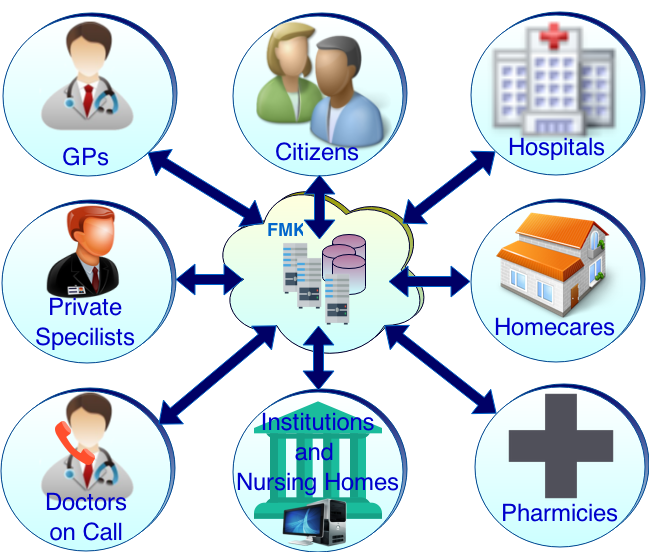
\includegraphics[width=0.7\textwidth]{./img/medicalcard.png}

	\caption{FMK general overview.}
	\label{fig:medicalcard}
\end{figure}

Not all treatments require prescriptions. I.e., the doctor can tell you to drink water, or take calcium tablets which you can get without a prescription, but he may make a prescription on these too. Everything prescribed will be in the system. Events are things that happen in the real world, such as a drug being administered to a patient by a nurse, or a drug being handed out at a pharmacy. 

The wide adoption of this system builds upon a successful cross--sectoral standardization of medicine workflows and closely related concepts. The system is not an electronic health record with specialized information such as test results, measurements or the like.

One of the primary design criteria for FMK is to provide high availability. The system is in use 24x7, and currently has 40+ integrations with other healthcare systems, most of which are required to use \gls{fmk} as the primary storage for relevant medicines data.

Though being simple at the high level, much of the challenge lies in making the system highly available, scalable and secure, supporting a wide range of use cases (as well as old \glspl{api}), all the while making sure that data that flows in from many of the connected systems has some measure of consistency. In many cases data ``updates'' are made on the basis of a previous``query'' to the system, and the system needs to have a model that captures conflicting updates. As such, this seemingly simple system ends up being surprisingly complex, especially because of the high availability requirement.

In context of making healthcare decisions, it is much better to have some information than none. It is better to have old information than none. Events that happen ``outside'' the system have indisputably happened, so the system needs to ingest them regardless of consistency.
All this leads us down the road to a \gls{crdt}-like data model deployed on Riak (dynamo-style eventual consistency w/write-conflict capture). The central patient information data model is essentially a stateful \gls{crdt}, that exposes a semantic model for write conflicts. Ideally, there would be a replica of the entire service+dataset in each major geographical region/hospital, which is still an eventual goal. Writes should be propagated ``as soon as possible'', but lack of such propagation - WAN failure - should not render the system unusable.

{\bf Network Topology and Architecture}: 
The system is made up of geographically separated data centers, set up in master-master replication mode, so any \gls{dc} can handle any request, Figure \ref{fig:system_overview}.
The client systems are systems providers for GPs and hospitals as well as a web based system that provides citizen access and acts as a backup for the professional systems.
Each client has affinity to a given primary \gls{dc}, so all requests from a given client use only one \gls{dc}, as long as it's available.
\begin{figure}[!h]
	\centering
	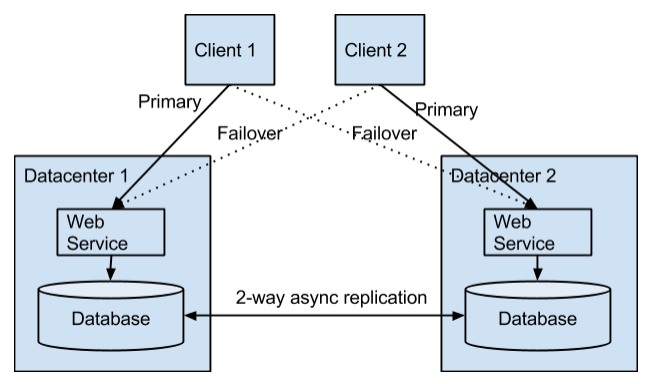
\includegraphics[width=0.8\textwidth]{./img/image3.png}

	\caption{System overview.}
	\label{fig:system_overview}
\end{figure}


\subsection{Conflict Situations}
Because of the asynchronous client system interfaces, and distributed data centers, two doctors can prescribe conflicting medicine to the same patient simultaneously. A real-life example of this is right after a patient is discharged from hospital and visits his GP. The medicines that a patient was prescribed in the hospital are sometimes carried over from the hospital patient journal to \gls{fmk} after his discharge, and can coincide with the prescription of new medicine by a GP.
Because the system is EC, it is not always visible, that all updates have not yet propagated throughout. This means that conflicts can be detected after the conflicting changes were made.
``Conflicting medicine'' may be multiple prescriptions of drugs containing the same active substance, or two drugs which interact poorly. Optimally, a doctor making or adjusting a prescription has full overview of the patient's existing prescriptions when she does so.

\subsubsection{Acting on Conflicts}
When developing the present implementation of materialized views, we found a need to detect Riak objects with conflicts (i.e. with siblings). Conflicts may appear in ways not triggered by client reads or writes, so objects which are seldomly or never read can exist for a long time in a non-resolved state. At present there is no mechanism for querying Riak for conflict-ridden objects and thus to consistently act on conflicts; a solution (in the form of a new feature) was suggested on the riak--users mailing list, using Riak \gls{2i}.
Alternatively, this problem might be solved on top of the proposed ``secondary messaging'', by allowing a conflict observer to be registered, e.g. on a per-bucket level.

\subsection{Invariants}
Since availability and partition tolerance are paramount, conflicts cannot be prohibited, but are instead corrected. There is no ``strong invariant'' in the system meaning the prohibition of data conflicts. The closest thing is that automatically resolved medicine cards must be marked as such (with a ``not reviewed'' flag) and stay so marked until reviewed and unflagged by a healthcare professional.
Prescriptions should not be created using medicines that is not on  the list of permitted medicines.

Merging multiple sets of prescriptions always converges towards the same set - no matter in which order the operations on the prescription set was done.
A single data center has read-your-writes consistency.

\subsubsection{FMK Merge}
One of the interesting issues in relation to SyncFree is how \gls{fmk} does merge, and which invariants need to be maintained.
In general, the system needs a \href{http://en.wikipedia.org/wiki/Bitemporal_data}{2-dimensional} temporal model, as it allows ``old versions'' to be updated to reflect that the system is not the truth. The truth is out in the real world. It could be that wrong information was entered into the system (maybe because a secretary entered information from an incomprehensible voice dictation), then the information is updated/decided upon by a third party, after which it needs to be possible to go back and correct the original input. Another possible conflict occurs in the case when a patient is involved in several treatments (at different facilities or with different health care professionals), but the drugs prescribed for these treatments have undesired interactions. Such ``drug incompatibilities'' cannot reliably be described as system invariants; they can to some degree be flagged by various external expert systems. In the end, the system can only flag non-causal updates, and let the domain professionals decide. One of our working rules when working with drugs is to not make decisions in code, but help the domain professionals to make the decisions.

The structure of a person record is a composite semi-\gls{crdt} like this:
\begin{itemize}
	\item person data (name, id, address, ...)
	\item treatments [\gls{crdt} set]
	\item prescriptions [set]
	\item prescription [stateful]
	\item prescription events [add-only]
	\item other events [add-only]
\end{itemize}

%(If you want to dive further into the exact model/merge, I'm sure we can dig out the actual Java code involved if someone wants to spend time understanding it.)

There is a life time on the order of a few years on all closed treatments; after this interval, they are deleted and no longer shown to users and client systems.

The core ``problem'' is what happens when a prescription record is updated w/ conflict, as it cannot be completely reconstructed from the corresponding ``prescription events'' (that might have been a better model to be completely ops-based). Prescriptions are not deleted but ``hidden'' (marked deleted). As mentioned above, in case of write conflicts, we do a ``best effort'' merge, and flag the record as in need of review. End-user systems are then required to visibly signal this status until a professional review has been performed.


\subsection{Transactions}
ACID transactions are avoided throughout the system, because of the high availability requirement.

A common use case involves a pharmacy querying for prescriptions that a patient will be picking up soon (prescriptions stored in the system can be tagged with a pharmacy where it is to be fulfilled). Since this is a very common query, we would like to be able to service such queries with a materialized view, rather than a coverage query which usually involves all machines in a cluster (Riak 2i). This however, is difficult as Riak provides no cross-object consistency.
The atomicity/consistency we need can be described as a delayed-consistency materialized view: whenever a pharmacy-prescription relation is added, updated or removed, that change will eventually — and within reasonable delay — be reflected in the view.
(This implicitly addresses the ``isolation'' part as well: seeing the updated prescription but an unupdated view is acceptable, especially since no high-level operation refers to both.)

Adding transactions to Riak would allow updating a materialized view like this, but at the same time reduce the availability, since an update now involves twice as many nodes. With more dependent updates, this can quickly require the most of cluster to be up to perform updates.
It would be very attractive — and a great research target — to have an alternative model for ``causally dependent updates'' in which events (ops in \gls{crdt}-terminology) could be reliably - albeit eventually - delivered to other entities inside the storage system, such sends being triggered by writes.

In the case in question, when a prescription is added/updated for a ``patient object'', imagine a reliable message  \textless add-prescription P \textgreater to the ``pharmacy object'' being enqueued as part of the update. The patient update operation can return success to the caller as soon as the message is reliably enqueued, as it is guaranteed that it will eventually be delivered to the ``pharmacy object'', even if the node(s) hosting it are currently inaccessible. Especially when the target of such an eventual, but reliably guaranteed, message is a \gls{crdt}, this model seems very attractive as an alternative to traditional transactions because it will in many cases be able to gracefully handle out-of-order delivery of ops.
  
Also, by avoiding transactions spanning multiple entities on the critical path this could lead to significantly better availability than a transaction based model.
A guaranteed message delivery system would requires some kind of transactions internal to the storage cluster, but those can be decoupled from the primary read/write operations. Issues can arise if too many messages end up being undelivered for an extended period of time.

A reliable messaging system is much easier to implement if the target of messages is known to be idempotent, because the system only needs to guarantee ``at-least-once delivery.''
The intersection of \gls{crdt}/messaging also brings to mind all the work being done in the area of \gls{cqrs}. Likewise, a good reference for inspiration in this area is Pat Helland's \hyperlink{http://www.ics.uci.edu/~cs223/papers/cidr07p15.pdf}{Life beyond Distributed Transactions: an Apostate's Opinion}. So, I propose we do research into a weaker consistency control mechanism based on \glspl{crdt} and reliable messaging as an alternative to transactions.

\subsection{Divergence}
\subsubsection{Expected latency}
There are different latency between data centers and between clients and data centers.
In normal operating mode, the latency between data centers should be below 5 minutes.
The \gls{dc}-client latency depends on the client system ranging from milliseconds to days.

\subsubsection{Offline mode}
In normal operation, a hospital can temporarily take ownership of a patients data, while he is admitted. When the hospital has this ownership, it operates offline, until it returns ownership to the central service.
In a failure scenario, some client systems must also be able to run offline without connection to a central service.

\subsubsection{Limits to the degree of temporary divergence}
For example, when a doctor prescribes a drug, the prescription should be in the pharmacy system before the patient arrive at the pharmacy to pick up the medicine. In practice, this seldom take less than 15 minutes, which is the delay that the system is engineered to support in the normal operating scenario.

\subsubsection{Divergence visibility}
It would be very useful to have an indication on how divergent the different components are for a given patient. When a doctor sees a patient's data, it is interesting to know if the latest data from for instance a hospital is present.
This could be represented by a timestamp for which the client knew that all other core--components had successfully completed replication of incoming data. 
There could always be delayed data from the unbounded set of peripheral client-systems. Ideally, there would be a timestamp available from all relevant components telling when they last synced data for this patient.

Probabilistic measurements on divergence would be relevant for the technical staff, but provide little direct value to end-users.

\subsubsection{Divergence guarantees}
For the usual high availability use cases of providing access to a patient's medication data, it would not be relevant to have mechanism that guarantee that data is not divergent because enforcing consistency requirements reduce availability.

For the offline data analytics use case, it could be relevant to wait with analyzing, until all data is guaranteed to be sufficiently up-to-date. A probabilistic value would be better than nothing, but would increase complexity, because late updates would need to be detected and handled by for instance redoing the analysis.

\subsection{Partitioning}
The fundamental level of consistency is the patient. Data is modelled per patient. 
In addition to that, client systems often fire off a string of operations on the same patient in a short interval of time, and need read-your-writes consistency. Therefore, the network is partitioned in data centers, such that a given client system is usually operating on the same network partition. Within this partition (data center) the system (almost) provides read-your-writes consistency. This is not the case for the global system.

\subsection{Operational Requirements}
\begin{itemize}
\item Reason for EC: Availability.
\item Where is the application running: in infrastructure, in a small number of data centers (~2-5).
\item How many replicas: ~5-20.
\item Full replication or partial replication: Full replication as for medicine cards.
\item The expected number of objects:
\begin{itemize}
\item Millions of medicine cards.
\item Millions of request-log entries (14-day history).
\item Billions of audit-log entries (a few years of history).
\end{itemize}
\item The expected sizes of objects:
\begin{itemize}
\item Medicine cards: On the order of 10KB.
\item Request-log entries: On the order of 10KB.
\item Audit-log entries: On the order of 1KB.
\end{itemize}
\item Total size of data set:    
\begin{itemize}
\item Medicine cards: On the order of 100GB.
\item Request log: On the order of 100GB.
\item Audit log: On the order of 1TB.
\end{itemize}
\item Rate of growth?
\begin{itemize}
\item Medicine cards: Unknown.
\item Request log: On the order of 10GB/day. Requests are deleted after 14 days.
\item Audit log: On the order of 100MB/day
\end{itemize}
\end{itemize}
\begin{itemize}
\item Partitioning of the database:
Given that any citizen can be treated in any part of the country at any time, the medicine card database can not as such be split into independent parts. On the other hand, no consistency is assumed across person IDs.
The set of objects is split into data of different flavors (domain data, write-twice request log for caching purposes, write-once access log for auditing purposes).
\end{itemize}

\subsection{Security Requirements}
%Doctors are not legally allowed to see ``any'' patient information but the system  does not block him. Access are logged to allow government operator to manage unallowed access.
Doctors are only allowed to see information regarding their patients however the system will not block access to other patients records. Nonetheless, access are logged to allow government operators to manage unallowed access.
\begin{itemize}
	\item Access control and granularity: There is an operation/rule matrix determining which operations are allowed for a user.
	\item As a main rule, there is no per-object access rule - any doctor or other health care professional can access any citizen's data at any time (as explained elsewhere). There is legislation, though, against accessing data for anyone who is not in your care at the time. Access can therefore be verified after-the-fact.
	\item Information flow control: all the operations produced in the system are logged and government operators access them to detect problematic behaviors. This management is done out of the actual system. 
	\item Auditing: An audit log is maintained.
	\item Rolling back offending updates:
	\begin{itemize}
		\item[] The domain contains an ``invalidated'' state for most entities where this could be relevant.
	\end{itemize}
\end{itemize}
Idea/Challenge \#1, Causally Dependent Updates

\subsection{Existing State}
This is a use case involving eventual consistency in Trifork production systems.

\subsection{On implementing 2m in Riak}
Here's some text for in Riak--speak describing how this could be done: ``2m: secondary messaging''. When an object is stored, it would be nice to be able to reliably deliver some message to a third party, e.g. to update a materialized view.
This could be done, much like 2i, by storing the ``intent to send'' as part of the same write that writes the object and the index. Then a post-commit hook will do the send, and when the message is acknowledged, the ``intent to send'' should be deleted at all participating nodes.
Overwriting an object does not overwrite/delete old ``intents to send''. A 2m subsystem will periodically scan for ``intent to send'' objects for which acknowledgments are past due, and re--transmit messages. Since intents are stored based on preflists, a ``preflist leader'' should be responsible for the intents pertaining to that preflist.
Delivered (acknowledged) messages need to be represented by a tombstone, or a similar mechanism.
These can be reaped on a per-preflist basis by keeping track of the oldest undelivered message in such a preflist, reaping intents that are older than that.
If the target of these messages are not just any message receiver, but an idempotent ops-based \gls{crdt} defined within the system, then re--transmits should be a non-issue. Sends to outside agents may never succeed delivery, but would still be an interesting use case.

\subsection{Other Challenges in FMK}
As part of the security policy, all operations are logged in an audit trail. This is what generates most of the data: the core dataset is on the order of 500GB, but the audit logs are an order of magnitude bigger.
The audit logs needs to be indexed for various usages. For example users (citizens) have online access to the audit trail for their own data, and part of the security model depends on after-the-fact review of audit logs. Some of these access patterns are best dealt with using analytics style batch processing, whereas online access to a user's own audit trail would be nicely dealt with using a causally dependent view as suggested above.

\subsection{Further Reading}
Source code for merging medicine cards \hyperlink{https://gist.github.com/rsltrifork/b1c648fe02bc0547389c}{Medicinecard Conflict Resolver} (source repository).

Danish doc on how merging is performed:
\url{https://docs.google.com/document/d/1uJw-GHvu380zgibG5_ZtFoCGYGszcPS7ykZR5DLiDW8/view#}

General public information on FMK (Danish)
\hyperlink{http://digitaliser.dk/group/1597792/profile}{Medicinecard}


\section{Music Festival App}

\subsection{Application Description}
This application intends to maintain participants of large event/gathering informed of the different activities in the event, progress and ratings for each of the acts as the event progresses. The participants may get this available information and take part in some of the voting activities, which generate the ratings, by using their own devices, e.g. smart phones, tables and laptops.

At large events where thousands of people gather, the internet-connection from mobile devices is often degraded to non-existent. Therefore, the Roskilde app is designed to function in a completely off-line scenario -- including the exchange of information. This is done on a P2P--basis (\gls{p2p}) by data synchronizing two devices using  direct communication based on bluetooth or wifi--direct.

This ``sometimes connected'' scenario, is a perfect match for \glspl{crdt}, and the Trifork Relai product, Figure \ref{fig:trifork_relai}.
\begin{figure}[!h]
	\centering
	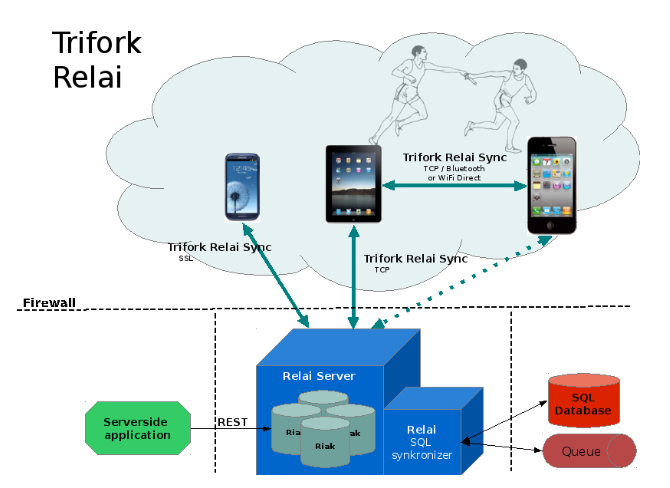
\includegraphics[width=0.9\textwidth]{./img/image4.png}

	\caption{Trifork Relai.}
	\label{fig:trifork_relai}
\end{figure}

\subsubsection{Requirements}
The app is extended with features each year. For the 2014 version, up- and down-votes for concerts has been suggested. Given the decentralized grid-type network topology, and the high number of devices, this use case would likely require aggregating the votes in order to achieve sufficient performance and to satisfy space requirements.
At the same time, sufficient information should always be present, so a vote is not counted twice. Because no user authentication exists in the app, every device with the app installed is considered an actor, and given a unique actor-id.
Good concerts will get positive votes, while bad concerts may end up with negative votes.

\subsubsection{Non-functional}
Roskilde Festival is a 2 week event, so the system should be massively available during this time, and in the days before. Afterwards, the system is very infrequently used until next year's festival. This gives special operational requirements and possibilities. I.e. long service windows outside the festival days have no impact.

The app must be very easy to use. For ease of use, no (additional) user registration or login process can be required from the user. 

\subsection{Conflict Situations}
Conflicts may arise, if the same information is updated from multiple devices. This has not yet been possible in this use case, as both user created content, and data pushed from the central server was immutable.

In the new up/down vote use cases, votes are cast from multiple devices on the same concert at the same time, giving different views on the performance of an artist.

\subsection{Invariants}
In the up/down vote use cases, a vote on a concert from an actor (device) must be counted precisely once. 
After data syncing two devices, all information from both should be present at both. 
However, if this is impractical due to physical constraints on data size and communication bandwidth, the amount of data transferred  could be limited. 

A proposed solution to limit the space is to exchange ``randomly'' only a part of the ``new'' information you get to the other peer. Somewhat related to lightweight probabilistic broadcast. In this case the invariant is that the combination of  the peers is correct. This also impact divergence that will be somewhat reduced.

For the actor counting votes, all votes should be included in the count, if they were either cast by the actor himself or other actors that have since synced with this actor after vote-casting. Votes should be relayed ``transitively'' through chains of syncs.

\subsection{Transactions}
No.

\subsection{Divergence}
The latency in offline mode is high, given that people need to enable synchronizing in their apps and be within range off pair-able devices.

Precisely measuring divergence in a master-less network with an unbounded set of devices that are joining and leaving all the time is at best difficult - possibly impossible. A probabilistic value would be fine.
A practical measurement could be number of nodes synced with in the last hour. I.e. counting the number of different devices that a given device has synced with, and that they have synced with a.s.o. for the last hour.

There are no limits to the allowable divergence, but perhaps there should be a warning, if the centrally pushed information is out of date.

\subsection{Partitioning}
People tend to group physically at a music festival, and there is a pattern of sleeping at night (or in the morning) , and being at the concerts during daytime.
The grouping of people in recurrent groups could potentially be used to dynamically structure the mesh network into a hierarchical, tiered network.
The advantage of a hierarchical model is the ability to have nodes handing off data to higher level nodes for aggregation, which would be very usable for votes for instance.

\subsection{Operational Requirements}
This application uses EC to be available during offline periods.
The application runs on mobile devices, connected - sometimes - to a central server.
Multiple data centers could in theory be used centrally, but this is not necessary given the load and offline capability.
Data is replicated to all participating devices, which are potentially one or more pr. festival guest. I.e. in the range of tens of thousands.
\begin{itemize}
	\item The number of objects could be a couple from each festival guest - I.e. hundreds of thousands. However, it has been much less so far.
	\item The object universe is flat.
\end{itemize}

\subsection{Security Requirements}
Because the app must be easy to use, no login is needed. Instead the app auto-generates a userid upon first startup.
Information flows freely between apps.
It is possible to centrally monitor the camp events sent, and delete inappropriate ones.

\subsection{Existing State}
The application is an existing app developed for Android and iOS. It allows festival participants to see the concert schedule and other centrally updated information as well as distribution of user-created content.


\section{\gls{b2b} Orders}
\subsection{Application Description}
It enables the shop employees to see a catalogue of upcoming clothes on a tablet device, and place orders on boxes for future delivery. This functionality is made available for the same shops to both shop staff as well as for shops managers, managers of chains of shops or managers of entire markets.
Orders are modelled as a \gls{crdt} Grow-only set (G-set), which is updated by adding event objects. Event objects are immutable, contain data and metadata about the event and can never be deleted. Example:
\begin{enumerate}
	\item[] Key:
	\begin{enumerate}
		\item[] shop123\_order234
	\end{enumerate}

	\item[] Events:
	\begin{enumerate}
		\item[] shop user 345 created an order for a box of pants

		\item[] order was received by serverXYZ and started processing

		\item[] order was rejected by serverXYZ because out of stock
	\end{enumerate}
\end{enumerate}

An overview of the current implementation of the system is shown in Figure \ref{fig:b2b_implementation}.
\begin{figure}[ht!]
	\centering
	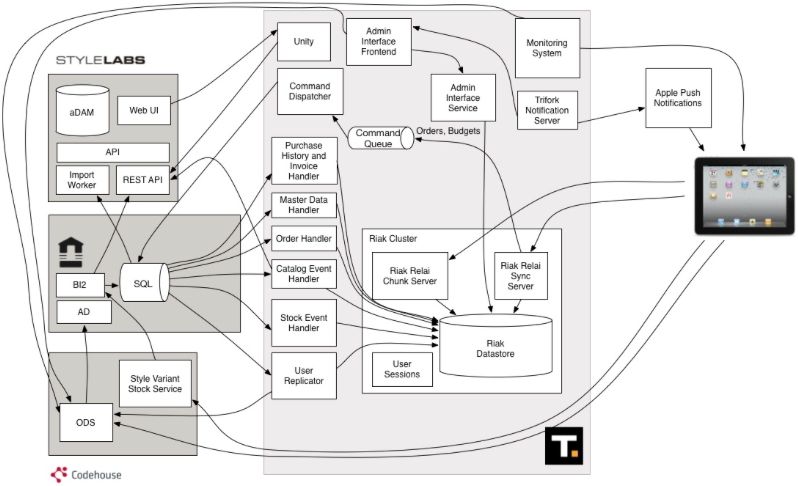
\includegraphics[width=1\textwidth]{./img/b2b.png}

	\caption{.}
	\label{fig:b2b_implementation}
\end{figure}

Causality tracking can be added by having each event point to the existing set of event-ids, that were already present when it was created. This event G-set model seems robust and general.

After a shop employee has given an order, it can be seen in the app, but no longer changed through the app, and if the shop employee want to cancel it or change anything, they need to contact the manufacturer customer support and ask them to fix it for them. The manufacturer can change an order by adding a new event to the order with the corrections, Figure \ref{fig:partial_data_replication}. The change depends on the current state of processing. I.e. if the boxes are already loaded on a truck and sent, fixing an incorrect order is different from fixing an order, that has not yet been processed.
\begin{figure}[!h]
  \centering
  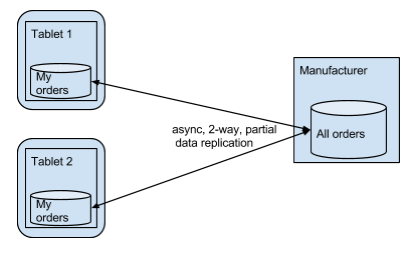
\includegraphics[width=0.7\textwidth]{./img/image5.png}

  \caption{Partial data replication.}
  \label{fig:partial_data_replication}
\end{figure}

\subsection{Conflict Situations}

When an employee creates an order on his tablet in offline mode, it is obviously not sent to the manufacturer until he is online again. Meanwhile, the item may go out of stock, or other employees ordering for the same shop, not knowing of this new order, can potentially order the same item again.
In theory, it is not possible to distinguish redundant orders. In practice, some rules can be applied to detect possible redundant orders - i.e. are they orders for the same item, approximately same number, same delivery date, and so on.

Manual resolution processes exist, which are based on contacting the manufacturer customer support.

\subsection{Invariants}
All employees related to the same shop, should always see an up-to-date picture of that shop's orders with respect to the data that is accessible after synchronizing devices.

% \subsection{Invariance} % As commented by Peter, this is a superfluous section.
Because we want to enable offline, we compromise on the invariant. It is ok to update the list of orders as soon as the information has been able to pass through the system.

\subsection{Transactions}
Shops also have a budget. When multiple employees order at the same time, they may exceed this budget. This is handled because the manufacturer back--end system serializes access to data for a given shop
.
Read-your-writes consistency is enforced by having a local replica on the tablet that is used for all local operations.
There is no cross-object consistency requirements for data generated on the tablet.
\subsection{Divergence}
The expected latency can be quite high because of the supported offline mode. An employee could take the shop ipad to his grandmothers house and place orders there offline, and not returning it until days after.
However, this will increase the risk of popular items being sold out.
A given catalog has an in-sale period, where orders are accepted. For practical manufacturing reasons, there must be some time between ordering and delivering, which is controlled by this period. If orders are not synchronized in before the end of the insale--period, they are likely not going to be accepted.

It is useful for the manufacturer to know when shop employees last synced their iPads. There is already some monitoring on this. A probabilistic value would not be useful for this.

It may be useful, to stop the shop employee from ordering more, if he has not synced with the central system for too long.

\subsection{Partitioning}
Currently there is no need for partitioning. Should the volume of requests increase or should there be a desire to run from multiple data centers, partitioning is an option.

The data is very centered around the shop domain object, and it would therefore be logical to partition data by shop. By keeping all operations on a given shop in one data center, divergence would be lowered.

\subsection{Operational Requirements}
This use case requires \glspl{crdt} to be available during offline periods.
The app is run on client controlled tablets connected to a single manufacturer controlled data center. The architecture is open for distributing to more data centers, should this become relevant.
Data is divided into buckets with different replication strategies. 
\begin{itemize}
\item Some data is general and go to all tablet
\item Some data is store specific - such as orders - and updateable from both client and server side
\item Some data is store-specific, but only updateable from the server. For instance store budgets.
\item Some data is store-specific, but only updateable from the client. For instance audit log.
\end{itemize}

Data modelling was made to give multistore managers access to a list of stores, and country managers to stores in a complete country.

We expect in the order of magnitude millions of objects with an avg. size of around 10k. Binary objects are divided into 64k blocks and streamed to the client with low priority.

The object universe is partitioned  into countries and stores.

\subsection{Security Requirements}
Access must be restricted so store employees can only see and update the information for their own store. Exceptions being country and multi-store managers who must be able to operated on multiple stores.

\subsubsection{Security Model}
When starting the app for the first time, the user is asked to log into a central token-issuing authority by providing userid/password. The token-issuer returns a signed response message stating the clients id and token expiry time.
When the client afterwards needs to sync restricted information from the central data-server or send any information to it, it must initiate the syncing protocol by sending its signed identity message. The data-server validates the signature using the token-issuers public key and builds the user context for later deciding if the user is authorized to the operations he is trying to do during the session.
In time before token expiry, the client automatically renews the token by providing the old token. This is also the point of a token revocation check.

\subsubsection{Data Poisoning Incident}
Due to a bug in an app build, invalid order data was injected into some apps. Upon syncing with the server, this invalid data was then propagated virally to the server and onward to other clients.
Additional security measures guarding the server's data would have been useful. Such security guards will likely be easier to implement using ops-based \glspl{crdt} than the current state-based model.
\subsubsection{Auditing}

The app creates a stream of audit information, which is synced to the server when there is a connection. In the server, this is indexed, and can be queried and aggregated on all contained data fields.

\subsection{Existing State}
This application was built from the ground up for a large clothes manufacturer, who sells boxes of clothes to thousands of stores in 30+ markets.
It replaces a manual process, where travelling salesmen visited the stores and presented physical clothing sample collections.

\chapter{Conclusion}
% \section{Conclusion}
To conclude the presentation of the use cases, we present the different research or practical challenges identified through the questionnaire answers (see Appendix A - Expectations for the Use Cases). Since one of the goals of \gls{wp1} is to provide such challenge to the other work packages, we present them distributed among the tasks of the \gls{wp1} to \gls{wp4}. Another goal of \gls{wp1} is to provide applications on which \gls{wp5} evaluation will be conducted. The use cases to support evaluation in \gls{wp5} will be selected after further formalization (deliverable D1.2). A summary of the main characteristics of the different use cases presented here is shown in Table \ref{tbl:metrics}.


\section{Task 2.1 -- Support for \glspl{crdt} at the server side}
\gls{crdt} at the server side, i.e. replication between a limited set of servers across some data centers, corresponds to small-scale full replication. Such servers are considered stable and powerful; also, the latency between them is usually limited. However, a partition can occur between data centers, and possible divergence must be resolved.   
The wallet use case adopts such a replication scheme. Indeed, for security reasons, the replication occurs only at the data center level.
The medical use case also considers only full replication between a limited set of data centers.

\section{Task 2.2 --   Support for \glspl{crdt} at points-of-presence}
In this task, the project will study partial-replication and \gls{crdt} composition protocols. Partial replication is applied in the ad-counting use case. The ad-servers and the live statistic nodes only have partial information of the total counts. The use case suggests a specific protocol that allows temporary errors and afterward applies correction.

\section{Task 2.3 --   Support for \glspl{crdt} at the edge}
Protocols elaborated in this task targets a large scale and dynamic setting. In the music festival use case, replication is achieved until the edge of the network (i.e. mobile devices), and edge devices must communicate with each other. The user devices are partial replicas that have degraded connectivity and no obvious stability. The number of devices considered here can be large, and peer-to-peer or group communication between devices is used to merge data and to obtain a global \gls{crdt}.
The shop ordering use case also considers a dynamic setting of replicas. The employees' tablets are not stable and can go offline. However the scale considered here is not large. 

\section{Task 3.1  --  \gls{crdt} object composition and transactions}
Need for guarantees in the presence of \gls{crdt} composition appears in wallet and medical use cases. The medical use case manages quite complex data that might be updated concurrently. The patient information, as well as the medication are composite elements, and there are relations between the data element managed, such as happens-before relationship between prescriptions. Events that modify several object at the same time (e.g. patient and pharmacy) occur and might be managed by \gls{crdt} transactions.
\gls{crdt} composition occurs also in the wallet use case that compose virtual money and vouchers. Transactions between users are not envisaged in the use case description but might be designed as research goal.   

\section{Task 3.2  --  Divergence control and quality-of-data}
The ad-counting use case is a typical example where divergence control and quality of data should be present. A degree of error in the data is tolerated, however the system should be aware of the quality of data. 
The music festival is another use case where divergence control can be useful. Indeed, a decision based on the vote should be taken only when the margin of error is below the margin of the vote. 
In the medical use case, knowing, for instance, that some data can be missing should also be very valuable.

\section{Task 3.3  --  Security}
Security is an important aspect of every use case. Data should not be easily corrupted or disclosed by an attacker. Moreover, in the medical use case security is paramount. Access control must be managed and the data must not be modified by an unauthorized person. The different users of the system (doctors, nurses, administrators) have different roles and should have different authorizations. Security is also achieved a posteriori, since an audit log is produced in order to allow the legal authority to check the data.
Security exigences are also explicitly stated in the wallet use case.  

\section{Task 4.1 --   Basic programming model}
The basic programming model addresses composition and abstraction of \glspl{crdt}, causality determination of \gls{crdt} operations, and object purging. Abstraction is useful for every use case data type. Composition is required in the wallet and medical use case. Causality is useful in the medical, the shop ordering and the wallet use cases. Causality determination allows to order correctly operations that affect the objects. For example, the operation that credits an amount has to be delivered before the debit operation.

\section{Task 4.2 --   Extended programming model}
The extended programming model addresses transaction support, causality management, stream-based dataflow, and garbage collection. 
Transactions are present in the medical use case. Causality management might be useful in use cases where causality determination occurs. For instance, in the medical use case, causality information - e.g. knowing that a prescription occurred after an other event - is very important; however traditional causality insurance - waiting before delivering the dependent operation - is not acceptable.        
Dataflow occurs in several use cases. Ad counting is a typical dataflow instance. Also, votes and decisions in the music festival, as well as shop orders and remaining manufacturer stock, can be considered as dataflow instances. 
Garbage collection is useful in any application to remove metadata introduced to manage consistency. However, it is more critical in use cases where operations occurs frequently and can be compressed into a global result. This is the case of the ad-counting, the votes in the music festival, and the successive scores in the leaderboard use cases.  

\section{Task 4.3 -- Final programming model}
The final programming model addresses scalability problems. Scalability is a concern of all use cases (except maybe the shop ordering one as presented here). The ad counts, the wallet transaction,  the medical events on the extent of a country, the online social activity in a music festival, and scores in mobile games are counted millions, and may be, for some use cases, billions, depending on the success of the applications. 


%
% The following two commands are all you need in the initial runs of your .tex file to produce the bibliography for the citations in your paper.
%\bibliographystyle{abbrv}
\bibliographystyle{notplainnat} % References list without URL or DOI
\bibliography{../syncFree}  % sigproc.bib is the name of the Bibliography in this case
% You must have a proper ".bib" file and remember to run:
% latex bibtex latex latex to resolve all references
%
% ACM needs 'a single self-contained file'!
%
\printglossaries

\appendix
\chapter{Expectations for the Use Cases}
\section{Use Case Requirements description}
\subsection{Purpose of this document}
Gather requirements for natural language use cases.
If you need certain aspects to be described, please write your questions here.
If you write use cases, please see here, what the descriptions should include.

\section{Extended Questionnaire}

\subsection{Existing state}
\begin{itemize}
\item Says if your application is already implemented and operated or not.
\item If already existing, express the main challenge encountered to develop, maintain and operate the application in term of each below items (conflict, invariant maintenance, operation performance, security threats …).
\end{itemize}

\subsection{Application description}
\begin{itemize}
\item Describe your application
\item Network topology/architecture.
Please add a principal network diagram to give a basic understanding of the actors, system components such as mobile devices or database servers and the communication patterns between them. I.e. synchronous calls, messaging, 1 or 2--way state synchronization.
\end{itemize}

\subsection{Conflict Situations}
\begin{itemize}
\item Can you identify conflict situations, where concurrent updates without synchronization might break invariants?
\end{itemize}

\subsection{Invariants}
\begin{itemize}
\item Can you identify the invariants of your application?
\item Should conflict or invariant violations be prohibited, or is it OK to correct them after the fact?
\item Do invariants need to be true at all times or only eventually?
\item if invariant violations are to be forbidden (instead of repaired), how important is for all replicas to be able to execute operation that might lead to invariant violation? 
(e.g. in the Rovio ad case, if we have 5 servers serving some given ad that must be shown 50 times, it is possible to assign 10 ad impressions to each site - this may lead to one server A ending ad impression much sooner than the others -- is this acceptable, or should server A be allowed more ad impressions by obtaining rights from other servers)
\end{itemize}

\subsection{Transactions}
\begin{itemize}
\item is there any need for updating more than one object atomically in your application? Why?
Please describe the example and explain why is it important for updates to be applied atomically.
\end{itemize}

\subsection{Divergence}
\begin{itemize}
\item What is the expected latency? 
\item Is there an ``offline'' mode?
\item Are there limits to the degree of temporary divergence allowed?
would it be interesting to know how divergent is the data you are reading (from the data in other replicas/data centers)? Please give examples.
\item If yes, what type of information would be useful - number of operations not observed, difference in the value observed, how long your data is old, some other?
\item if yes, could you live with a probabilistic value (e.g. there is 90\% chance that you are not missing more than 3 operations)?
\item Would it be interesting to include a mechanism that guarantees that data is not divergent by more than some amount?
\item If yes, what type of information would be useful - number of operations not observed, difference in the value observed, how long your data is old, some other?
\item if yes, what price would you be ready to pay for it - increased latency on reads, increased latency on writes?
\item If yes, could you live with a probabilistic value?
\end{itemize}

\subsection{Partitioning}
\begin{itemize}
\item Does natural partitions exist in the system, such that global consistency can be lowered while upholding a higher degree of consistency the partitions? For instance if all data in a partition is handled by the same data center, then it can benefit from reduced latency between members of the same partition, and thus increased consistency.\\
Another example: Tiered data--handoff, where a hierarchy is made of nodes on different levels.
\end{itemize}

\subsection{Operational Requirements}
\begin{itemize}
\item Why do they require EC?  For availability?  Performance?  Scalability?
\item Where is the application running: on client-controlled mobile machines or in the infrastructure? If the latter, in a small number of data centers, or in large numbers of \glspl{dc}?
\item How many replicas: tens?  thousands?  millions?
\item Full replication or partial replication?
\item What is the expected number of objects: thousands? millions? billions?  Size of each object?  size of the data: bytes? megabytes? gigabytes?  Rate of growth?
\item Is the object universe partitioned (ie composed of discrete, independent databases that can be managed/replicated independently) or (one single big database)?
\end{itemize}

\subsection{Security Requirements}
\begin{itemize}
\item Access control?  at what granularity (object, operation, operation+arguments, user)?
\item Information flow control?  at what granularity?
\item Auditing + rolling back offending updates a posteriori?
\end{itemize}


\chapter{Other information}
\section{Summary of use cases}
The Table \ref{tbl:metrics} shows a summary of some of the values encountered in the use cases presented in this document.

\begin{landscape}
	\small  % Switch from 12pt to 11pt; otherwise, table won't fit
	\begin{center}
		 \begin{longtable}{|p{2.2cm}||p{3.6cm}|p{3.4cm}|p{3.4cm}||p{3.8cm}|p{3.4cm}|p{3.1cm}|}
			\hline
			Provider & 
				\multicolumn{3}{c|}{Trifork} & 
				\multicolumn{3}{c|}{Rovio} \\ \cline{2-7}

			     & 
				FMK & 
				Music Festival & 
				B2B & 
				Leaderboard & 
				Virtual Wallet & 
				Ad Counting \\
			\hline
			\hline
			\endhead
			\hline \multicolumn{7}{r}{\textit{Continue on next page}} \\
			\endfoot
			\endlastfoot

			No. DCs	& 
				Currently 2. Potentially more.	& 
				Normally 1 but many could be used & 
				1 DC but many could be used & 
				1 DC but many could be used & 
				1 DC but many could be used	& 
				1 DC but many could be used \\\cline{3-3}
	
			       & 
			       & 
			     Server and all mobile devices  & 
			       & 
			       &  
			       & \\
			\hline
	
			Replication & 
				Full & 
				Full & 
				Partial. Only orders from stores relevant to the user are replicated & 
				Full & 
				Full & 
				Full \\
			\hline
	
			No. Replicas & 
				Each DC has a Riak clusters with 3 replicas of each key. In addition a datawarehouse exists with one replica & 
				Thousands & 
				Stores are replicated to all users with access to the store. This is done when the user starts the app & 
				3 within a database	& 
				3 within a database	& 
				3 within a database but copies in cache increases to thens \\
			\hline
	
			No. expected of objects & 
				Millions of medicine cards. ~2 billion auditlog entries & 
				A couple per guest. Up to 70.000 guests & 
				Millions of orders & 
				(users $/$ 30) $*$ numberLevels & 
				Tens of hundred of millions &
				Tens of thousands \\ \cline{2-5} \cline{7-7}
			
				 & 
				Millions of request-log entries and 14-day history & 
				From tens of thousands & 
				10s--100s of million of auditlog entries & 
				A game with 100 levels and 300 million users generate 1 billion objects & 
				 & 
				May increase up to hundreds of thousands \\ \cline{2-3} \cline{4-5} \cline{7-7}
	
				 & 
				Billions of audit-log entries and a few years of history & 
				To hundred of thousands &
				 & 
				Many games running at a time so hundreds or millions or billions & 
				 & 
				Many counters aggregated into a single document \\
			\hline
	
			Partitioning of data & 
				Riak shards data in 256 partitions based on consistent hashing & 
				Riak shards data in 64 partitions based on consistent hashing & 
				Riak shards data in 64 partitions based on consistent hashing & 
				No & 
				No & 
				No \\
			\hline
	
			Object sizes & 
				Medicine cards: On the order of 10KB-1MB &
				 & 
				Average 10KB & 
				150 bytes & 
				From ~ 1KB & 
				Bytes \\ \cline{2-2} \cline{4-4} \cline{6-6}
	
				 & 
				Request-log entries: On the order of 100KB & 
				 & 
				\multirow{2}{3.4cm}{Binary objects bigger and streamed in chunks of 64K} & 
				 & 
				To tens of KB & 
				 \\ \cline {2-2}
	
				 & 
				Audit-log entries: On the order of 1KB & 
				 & 
				 & 
				 & 
				 & 
				  \\
			\hline
	
			Total size of data set & 
				Medicine cards: On the order of 100GB & 
				 & 
				0.1 to 1 TB auditlogs and 10GB orders & 
				150 GB & 
				30 GB & 
				200 KB \\ \cline{2-2}
	
				 &
				Request log: On the order of 100GB & 
				 & 
				 & 
				 & 
				 & 
				  \\ \cline{2-2}
	
				 & 
				Audit log: On the order of 1TB & 
				 & 
			 	 & 
			  	 & 
			 	 & 
				  \\
			\hline
	
			Rate of growth &
				Proportional to population growth in Denmark (very low) &
				& 
				& 
				& 
				& 
				 \\ \cline{2-2}
	
				 &
				Request log: On the order of 10GB/day. Requests are deleted after 14 days & 
				 & 
			 	 & 
			 	 & 
			 	 & 
				  \\ \cline{2-2}
	
				 & 
				Audit log: On the order of 100MB/day & 
				 & 
				 & 
				 & 
				 & 
				  \\
			\hline
	
			Consistency & 
				No consistency is assumed across person IDs & 
				Eventual consistency & 
				Eventual consistency & 
				Eventual consistency & 
				\multirow{2}{3.6cm}{Lower global consistency and higher consistency within DC (Strong Consistency)} & 
				Eventual consistency \\ \cline{2-2}
	
				 & 
				Eventual consistency & 
				 & 
				 & 
				 & 
				 & 
				  \\
			\hline
%		\end{tabular}
		
			\caption{Summary of values.}
			\label{tbl:metrics}
		\end{longtable}
	\end{center}
%	\end{table}
\end{landscape}


% So we can have the number of pages
\label{LastPage}
\end{document}
